%************************************************
\chapter{Validation and Performance Evaluation}\label{ch:validation}
%************************************************

In this chapter, we will describe the deployment of three testing scenarios: a laptop, a Raspberry Pi 3, and a Omega2 IoT device with the Raspberry Pi 3 as the delegation server. We will measure and compare the results to determine if the proposed solution is feasible or must be submitted to revision.

\section{Testbed description}

First, we shall describe the example Attribute Based Credential system in use. Then, the hardware we will use in our benchmarking.

\subsection{P2ABCE setting}

To test the correct execution of the \textit{IoT smart card}, we will use the ABC system from the tutorial in the P2ABCE Wiki\footnote{\url{https://github.com/p2abcengine/p2abcengine/wiki/}}. It is based on a soccer club, which wishes to issue VIP-tickets for a match. The VIP-member number in the ticket is inspectable for a lottery, ie. after the game, a random presentation token is inspected and the winning member is notified.

First the various entities are \textbf{setup}, where several artifacts are generated and distributed. Then a ticket credential containing the following attributes is issued:

\begin{verbatim}
First name: John
Last name: Dow
Birthday: 1985-05-05Z
Member number: 23784638726
Matchday: 2013-08-07Z
\end{verbatim}

During \textbf{issuance}, a \textit{scope exclusive pseudonym} is established and the newly issued credential is bound to this pseudonym. This ensures that the ticket credential can not be used without the smart card.

Then \textbf{presentation} is performed. The \textit{presentation policy} specifies that the member number is inspectable and a predicate ensures that the matchday is in fact $2013-08-07Z$. This last part ensures that a ticket issued for another match can not be used.

The ticket holder was lucky and his presentation token was chosen in the lottery. The presentation token is therefore inspected.


\hfil

\subsection{Execution environment}

First we will execute the test in our development machine (laptop). After asserting that the services work as expected, we then run the test in a Raspberry Pi 3, exactly like in the laptop. Finally, we will deploy the IoT smart card in a Omega2 and the delegation services in the Raspberry Pi 3. After every test, we checked that the issuing and proving were successful, in case a cryptographic error appeared in the implementation. 

Lets have a closer look at the hardware of each device:


\paragraph{Development laptop}\marginpar{
	\vskip0pt
	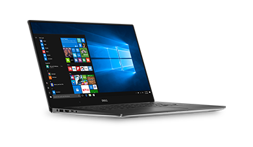
\includegraphics[width=0.8\linewidth]{gfx/DELL}
	
	DELL XPS 15
}
Our device is a DELL XPS 15, with a Core i7-6700HQ at 3.5GHz quad core processor and 32GB of DDR4 RAM, running Ubuntu 16.10.

This is a powerful machine that can simulate the performance of many servers and clients that would implement P2ABCE in a real environment, giving a reference point for performance comparisons.

\paragraph{Raspberry Pi 3}\marginpar{
	\vskip0pt
	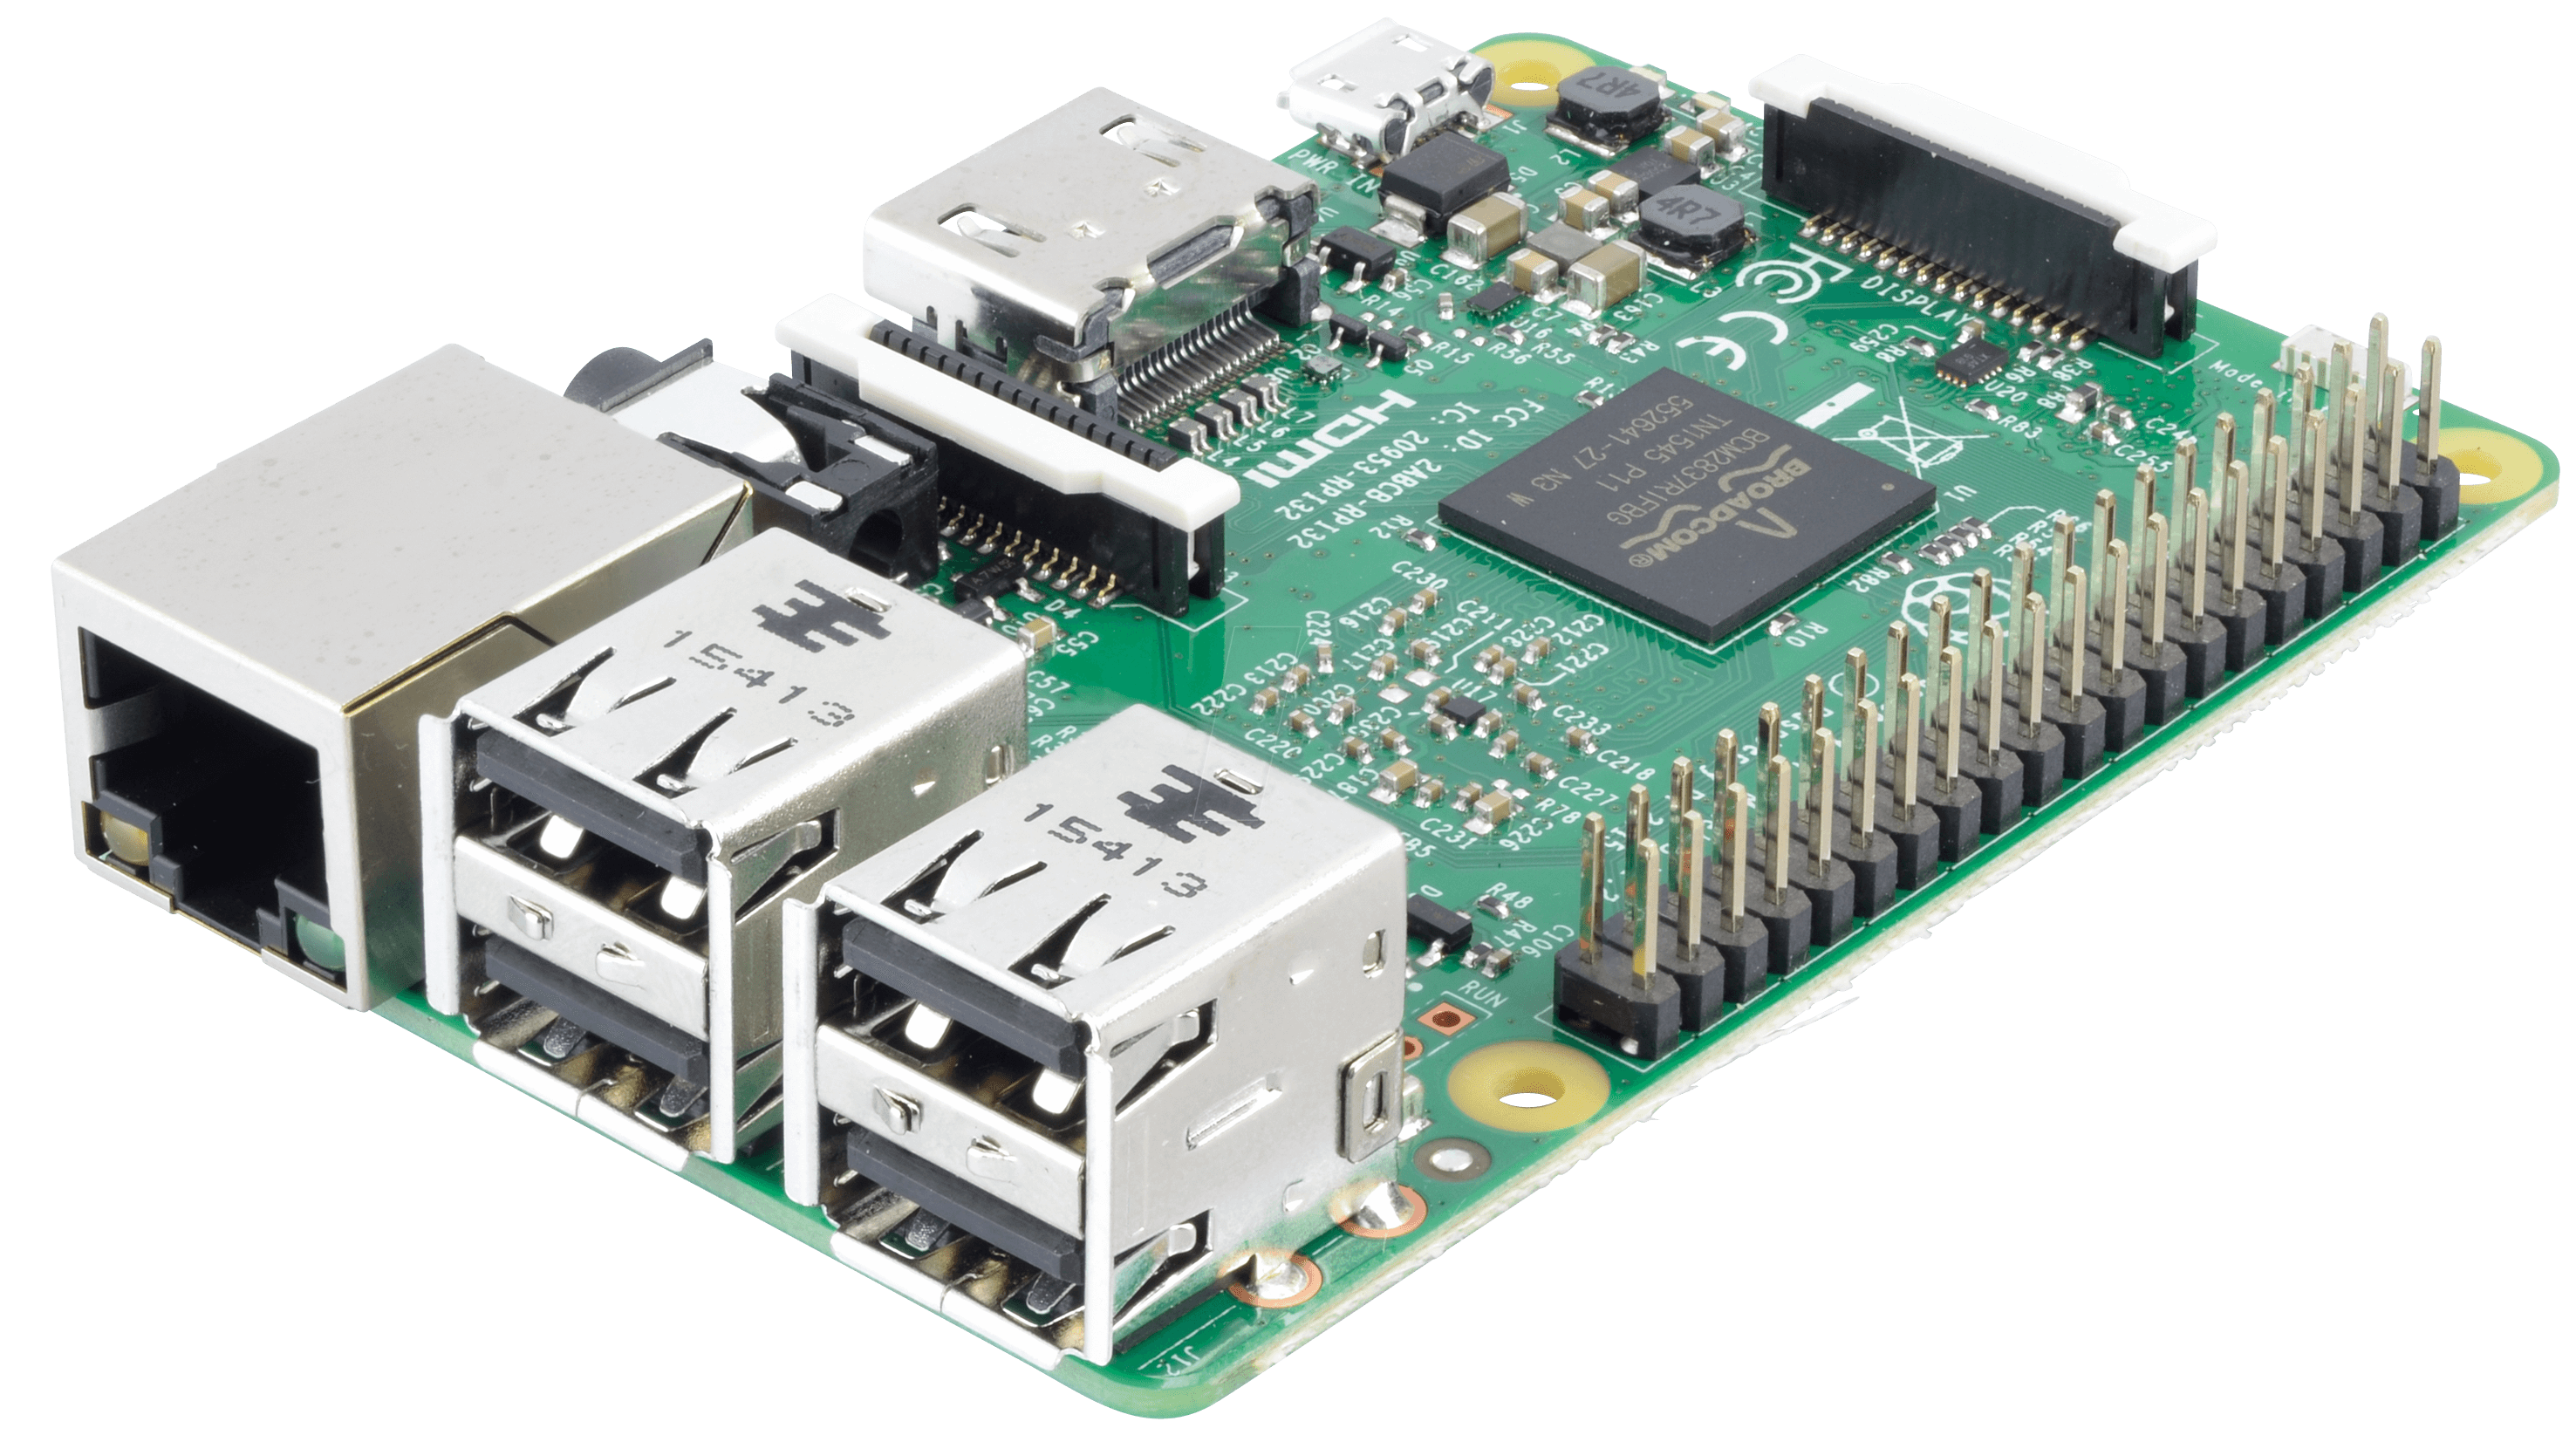
\includegraphics[width=0.8\linewidth]{gfx/RPi3}
	
	Raspberry Pi 3
} A familiar environment, powerful enough to debug and hold the delegated P2ABCE Java services of P2ABCE with its 1GB of RAM, and with two network interfaces, perfect to work as the gateway for the IoT devices to the Internet.

Only a microSD with enough space to burn the OS is needed to plug\&play with the Raspberry Pi. We use Raspbian, a stable Debian based distro, recommended by the Raspberry Pi designers, and ready to use with the P2ABCE compiled \textit{self-contained .jar} services.

\begin{table}[h]
	\myfloatalign
	\begin{tabularx}{0.75\textwidth}{ll} \toprule
		CPU & ARMv8 64bit quad-core @1.2GHz \\
		RAM & 1GB \\
		Storage & microSD \\
		Firmware & Raspbian (Debian based distro) \\
		Connectivity & Wifi n + Ethernet \\
		Power & 5V 2A \\
		\bottomrule
	\end{tabularx}
	\caption[Raspberry Pi 3 Specifications]{Raspberry Pi 3 Specifications.}
	\label{tab:RPi3Specs}
\end{table}


\paragraph{Onion Omega2}\marginpar{
	\vskip0pt
	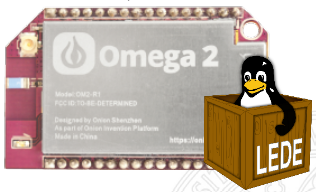
\includegraphics[width=\linewidth]{gfx/Omega2}
	
	Onion Omega2
} A device that falls inside the category of IoT, powerful enough to run a Linux embedded environment, such as LEDE, where we can develop and debug the first PoC without troubling ourselves with problems not related to the project itself.


\begin{table}[h]
	\myfloatalign
	\begin{tabularx}{0.75\textwidth}{ll} \toprule
		MCU & Mediatek MT688\footnote{MediaTek MT7688 Datasheet - \url{https://goo.gl/kqD2gF}} \\
		CPU & MIPS32 24KEc 580MHz \\
		RAM & 64MB \\
		Storage & 16MB \\
		Firmware & LEDE (OpenWRT fork distro) \\
		Connectivity & Wifi b/g/n \\
		Power & 3.3V 300mA \\
		\bottomrule
	\end{tabularx}
	\caption[Onion Omega 2 Specifications]{Onion Omega2 Specifications.}
	\label{tab:Omega2Specs}
\end{table}



Nonetheless, the Omega2 needs fine tunning to start operating, and basic knowledge of electronics to make it work. The two main things to begin with Omega2 are:
\begin{itemize}
	\item A reliable 3.3V with a maximum of 800mA power supply, e.g. a USB2.0 with a step-down circuit, with quality soldering and wires to avoid unwanted resistances. The Omega2 will usually use up to 350mA, when the WiFi module is booting up. The mean consumption is about 200mA.
	\item A Serial to USB adapter wired to the TX and RX UART pins to use the Serial Terminal, to avoid the use of SSH over WiFi.
\end{itemize}

A downside of using LEDE and the Omega2 is the lack of hardware acceleration for cryptographic operations, unlike the MULTOS applications, because the smart cards hardware and MULTOS API include support for such common operations in smart cards.



\paragraph{The network} In our third scenario, the Raspberry Pi 3 and the Omega2 will talk to each other over TCP. This implies possible network delays depending on the quality of the connection. The Raspberry Pi 3 is connected over Ethernet to a switch with WiFi access point. The Omega2 is connected over WiFi n to said AP. To ensure the delay wasn't significant, we measured 6000 APDU messages, and the results show that the mean transmission time is less than half a millisecond per APDU. As we will see in the results section, this network time is negligible.

\paragraph{Future work for tests} The lack of a physical MULTOS smart card precludes us to load and test the ABC4Trust Card Lite's code and measure the time P2ABCE would need when using the \textit{HardwareSmartcard} class. This would be really interesting because for a single method from the \textit{Smartcard} interface, \textit{HardwareSmartcard} implementation needs to send multiple APDU Commands, but \textit{SoftwareSmartcard} can perform the operations immediately, with the full computer's resources. Also, physical smart cards benefit from hardware acceleration in most of the cryptographic operations, unlike our software implementations in the PoC.




\section{The test code}

In this section we present the scripts and binaries used during the tests.

There are three pieces of software that conform the test: the P2ABCE services, the IoT smart card, and shell scripts automatizing the REST calls, from the terminal.

\paragraph{P2ABCE services}\hfil

This is a common part to our three sets. The services are compiled in a self-contained Jetty web server, or in WAR format, ready to be deployed in a server like Tomcat. We use the same JAR files with the embedded Jetty web server for the PC and Raspberry Pi.

We modified the User Service code to measure the execution elapsed time for each REST method. We don't measure the time the web server spends processing the HTTP protocol and deciding which Java method to call.


\paragraph{IoT smart card}\hfil

Our C implementation of the P2ABCE smart card, compiled for the Omega2, with BIOSC listening on port 8888 for the APDU messages.

We tested the execution in two modes, a full logging where every step was printed in terminal, and another one with no logging. With the first mode, we can check a proper execution, every byte exchanged, and with the second one, we measure the execution without unnecessary I/O.

\paragraph{Shell scripts} \hfil

To orchestrate all the services we use shell scripts that execute the REST calls using  \texttt{curl}. Here we perform the mentioned steps: setup of the P2ABCE system, issuance of the credential and proving for the presentation policy.

In the setup, the system parameters are generated, indicating key sizes of 1024 bits, the ones currently supported by the ABC4Trust and IoT smart cards. Then the system parameters and public keys from the services (issuer, inspector, revocation authority) are also exchanged and stored in each Service.

During the issuance and proving, the User and the Issuer and Verifier exchange multiple XML files, with the cryptographic information of each step of the Idemix protocol.


We offer two versions for the scripts. The first one is a single shell script file, to be executed from a single terminal. The advantage of this version is that, because every XML file is stored in the machine running the script, we don't have to transfer these files by other means, e.g. \texttt{scp}. An excerpt of this script showcases how we receive an XML file from the User Service, e.g. \texttt{secondIssuanceMessage.xml}, and send it to the Issuer Service, referencing the file stored in the script's working directory:

\begin{lstlisting}[language=bash]
[...]
# First issuance protocol step - UI (first step for the user).
echo "Second issuance protocol step (first step for the user)"
curl -X POST --header 'Content-Type: text/xml' -d @uiIssuanceReturn.xml 'http://localhost:9200/user/issuanceProtocolStepUi/' > secondIssuanceMessage.xml

# Second issuance protocol step (second step for the issuer).
echo "Second issuance protocol step (second step for the issuer)"
curl -X POST --header 'Content-Type: text/xml' -d @secondIssuanceMessage.xml 'http://localhost:9100/issuer/issuanceProtocolStep/' > thirdIssuanceMessageAndBoolean.xml
[...]
\end{lstlisting}


The second script version is intended for a more realistic execution. In a real scenario, the User and the Issuer, for example, would call the REST methods of their respective Services, but not the other actor's Service, exchanging the XML files through other means. Instead of one script running in a single machine, orchestrating the Omega2, Raspberry Pi 3 and laptop, we offer three scripts, one per machine, with \textit{pauses} where one device must send an XML file to another machine. An excerpt from the Omega2's script shows the same step as above, but instead of calling the Issuer's REST Service, waits until we send the corresponding files.

\begin{lstlisting}[language=bash]	
# First issuance protocol step - UI (first step for the user).
echo "Second issuance protocol step (first step for the user)"
curl -X POST --header 'Content-Type: text/xml' -d @uiIssuanceReturn.xml "http://$Rpi3IP:9200/user/issuanceProtocolStepUi/" > secondIssuanceMessage.xml

read -p "Send => secondIssuanceMessage.xml <= back to the Issuer. Then press any key to continue... " -n1 -s

read -p "Receive => thirdIssuanceMessageAndBoolean.xml <= from the Issuer. Then press any key to continue... " -n1 -s
\end{lstlisting}


\hfil

The first version is recommended for tests, and the second version only for instructive purposes.


\section{Results}

After 20 executions for each scenario (laptop, RPi3, Omega2+RPi3), we take the means and compare each step of the testbed.

It is worth noting that during the test, the measured use of the CPU showed that P2ABCE does not benefit of parallelization, therefore, it only uses one of the four cores in the laptop and Raspberry Pi 3.

To test the network, we sent six thousand APDUs to the Omega2, but instead of calling the \textit{APDU handler}, the Omega2 responded with the same bytes back. This way, the Omega2 only performed the simple BIOSC protocol, reading from and writing to the TCP socket.
The APDUs had multiple sizes, taken from the most common APDUs logged in during a successful execution. The test showed that our network speed was around $0.014$ ms per byte.


\paragraph{The setup}\hfil

The first step of our testbed. The Omega2 doesn't intervene until the creation of the smart card, therefore, the times measured in the second and third scenarios are practically identical.

\begin{figure}[bth]
	\myfloatalign
	\subfloat[Times and relative speedup]
	{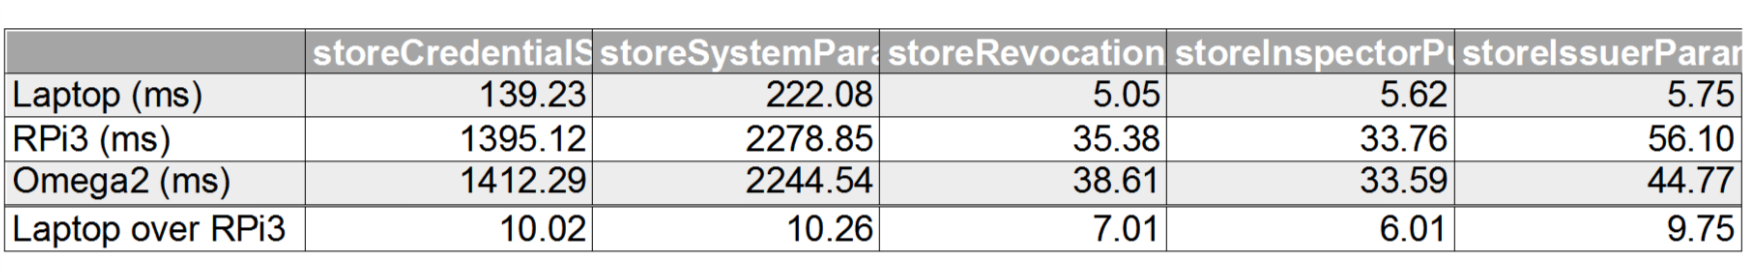
\includegraphics[width=\linewidth]{gfx/graphics/setuptable}} \quad
	\subfloat[Comparison graph]
	{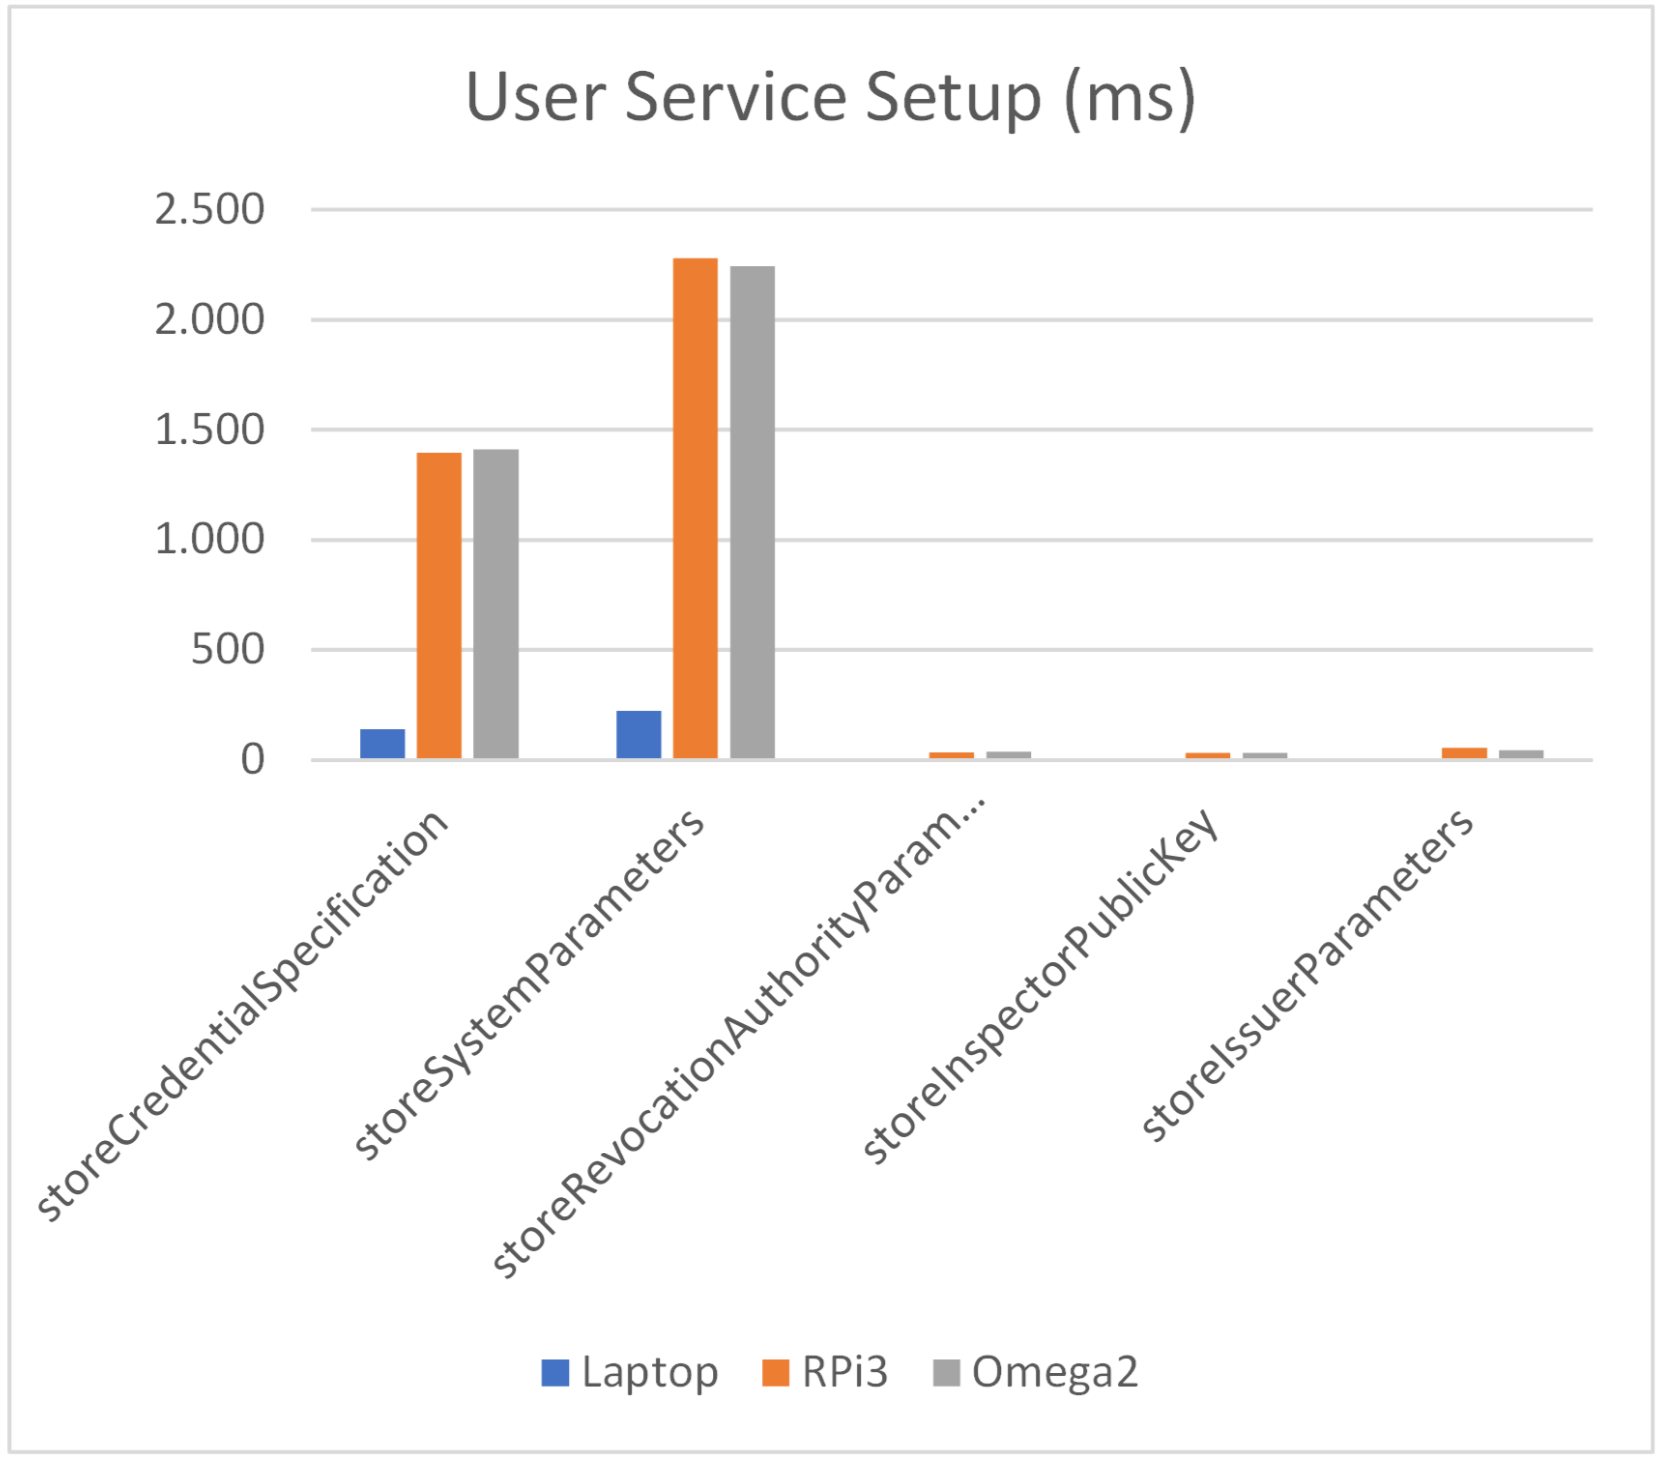
\includegraphics[width=.8\linewidth]{gfx/graphics/setup}} \\
	\caption{Setup times (milliseconds)}
	\label{fig:setup:graph}
\end{figure}

As we can see in \autoref{fig:setup:graph}, the laptop is about ten times faster than Raspberry Pi 3, but considering that the highest time is less than two and a half seconds, and that the setup is done only once, this isn't a worrisome problem.

\paragraph{Creation of the smart card}\hfil

Here we create a \textit{SoftwareSmartcard} or a \textit{HardwareSmartcard} object that the User service will use in the following REST calls.

The REST method to create a \textit{SoftwareSmartcard} is $/createSmartcard$, and to create a \textit{HardwareSmartcard}, using the \textit{IoTsmartcardio} implementation, we use $/initIoTsmartcard$. This operation is done only once per device, and includes commands from the creation of the PIN and PUK of the smart card, to storing the system parameters of P2ABCE, equivalent to the previous setup step.


\begin{figure}[bth]
	\myfloatalign
	\subfloat[Times and relative speedup]
	{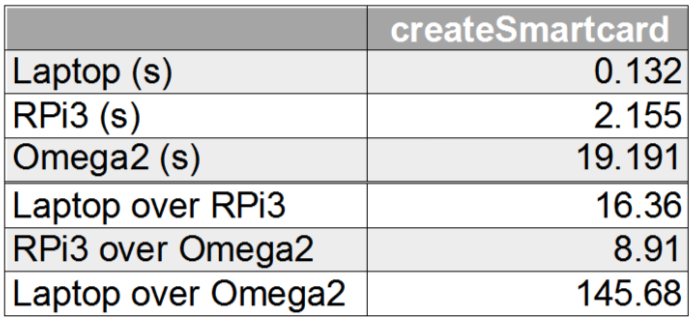
\includegraphics[width=0.5\linewidth]{gfx/graphics/createSCtable}} \quad
	\subfloat[Comparison graph]
	{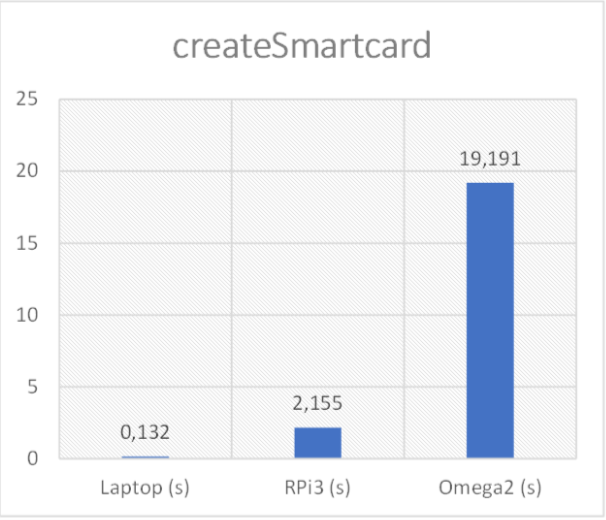
\includegraphics[width=0.45\linewidth]{gfx/graphics/createSC}} \\
	\caption{Create smart card times (seconds)}
	\label{fig:createSmartCard:graph}
\end{figure}

From \autoref{fig:createSmartCard:graph} we see that the RPi3 is about 16 times slower than the laptop in the creation of the \textit{SoftwareSmartcard}, but almost 9 times faster than the setup of the smart card in the Omega2 using APDUs. This gives us that the laptop is 145 times faster than the combination of RPi3 and Omega2 in our IoT deployment.
But looking at the times, this process lasts up to 20 seconds, making it something feasible.

This is the first interaction between the RPi3 and the IoT smart card running in the Omega2. To setup the smart card \textbf{30 APDU Commands}, and their respective Responses, are exchanged, as shown in \autoref{ch:resultsdiagrams}, \autoref{fig:APDUsInitIoTSC}, with a total of $1109$ bytes. From our network benchmark, using TCP sockets, the delay in the transmission is only around 15 and 20 ms, negligible, as we said, compared to the almost 20 seconds the operation lasts.


\paragraph{Issuance of the credential}\hfil

Our credential will have 5 attributes and key sizes of 1024 bits, as specified during the setup process.

The issuance is done in three steps for the User service, shown in \autoref{fig:IssuanceInteraction} with a red note showing the start of each step for the User delegation, in green for the interactions between Issuer and User, and the darker red is the Identity service, choosing the first available identity to use. The arrows in the figure show the REST calls performed during the test, where the IoT device acts as User, the RPi3 hosts the P2ABCE delegation services and the laptop is the Issuer.

The three delegation steps and the REST method called are:

\begin{center}
	\begin{tabular}{l|l}
	First issuance protocol step & $/issuanceProtocolStep$ \\
	Second issuance protocol step  & $/issuanceProtocolStepUi$ \\
	\textit{(end of first step for the User)} & \\
	Third issuance protocol step & $/issuanceProtocolStep$ \\
	\textit{(second step for the User)}  & \\
\end{tabular}
\end{center}


\begin{figure}[bth]
	\begin{center}
		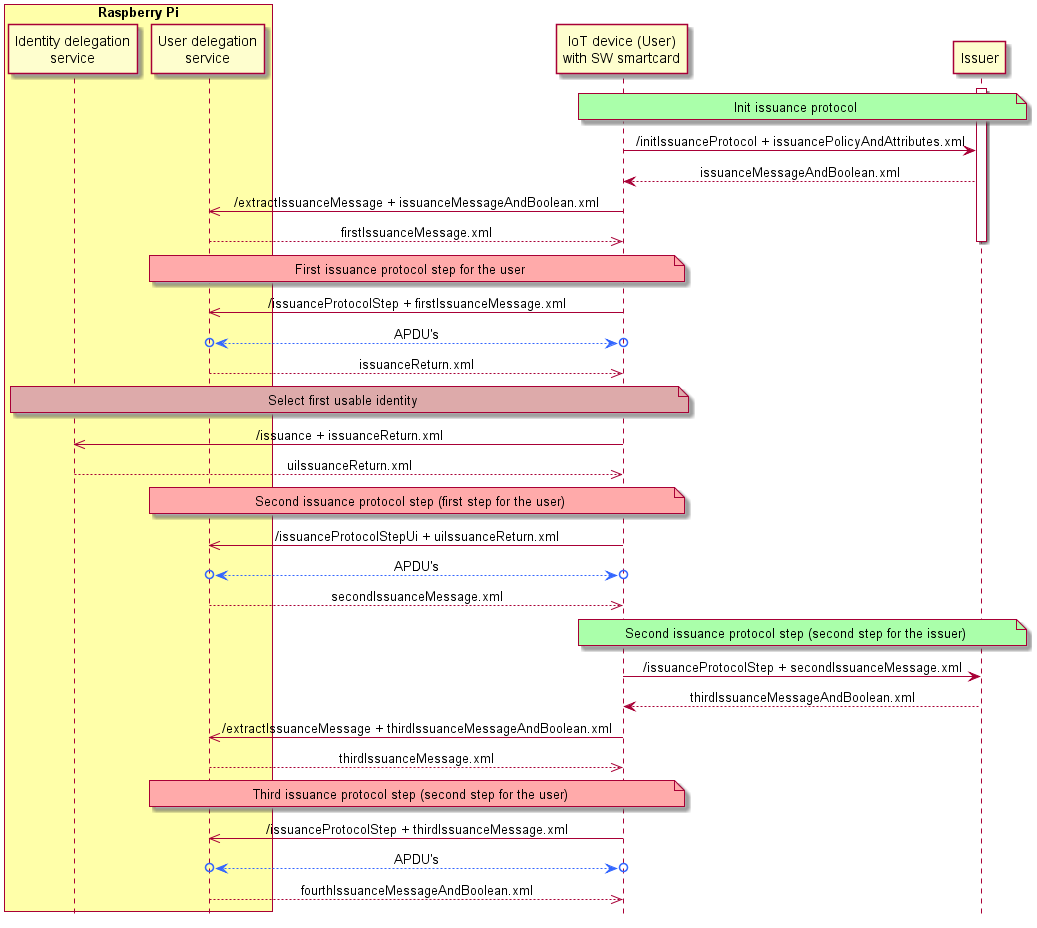
\includegraphics[width=\linewidth]{gfx/UML/IssuanceInteraction}
	\end{center}
	\caption{Issuance interaction.}
	\label{fig:IssuanceInteraction}
\end{figure}



As we can see, the three REST calls to the delegation User service involve communication with the smart card. We show in \autoref{ch:resultsdiagrams}, \autoref{fig:IssuanceAPDUs}, the APDU Commands used for each REST call in the issuance.
There are 45 APDU Commands in total, $3197$ bytes exchanged, that would introduce a latency of 45ms in the network, negligible.


\begin{figure}[bth]
	\myfloatalign
	\subfloat[Times (ms) and relative speedup]
	{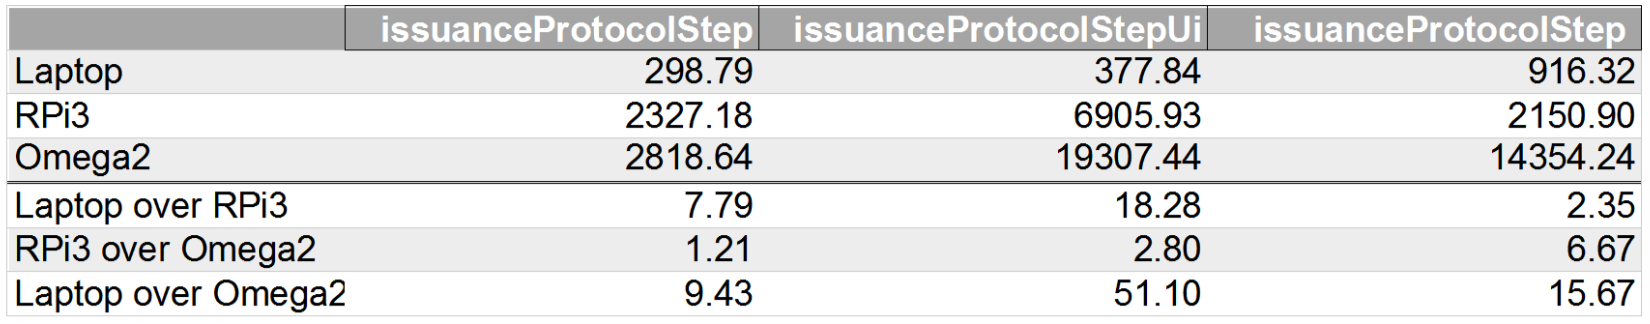
\includegraphics[width=\linewidth]{gfx/graphics/issuancetable}} \quad
	\subfloat[Comparison graph]
	{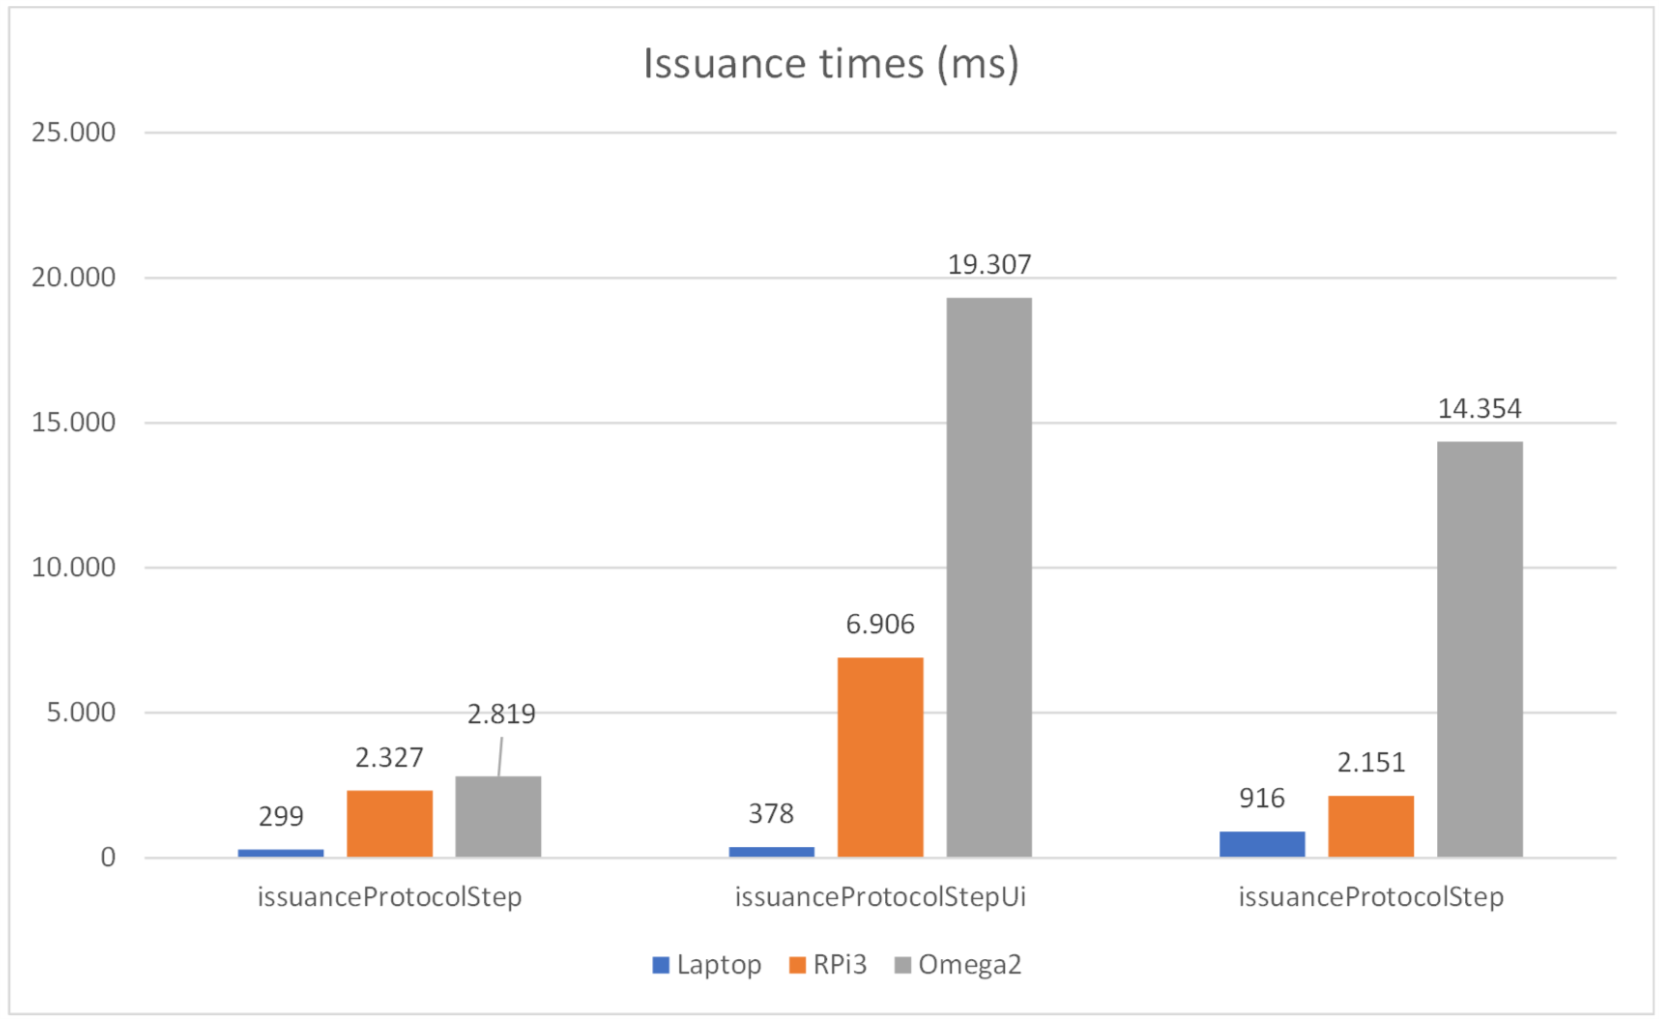
\includegraphics[width=.8\linewidth]{gfx/graphics/issuance}} \\
	\caption{Issuance times (milliseconds)}
	\label{fig:issuance:graph}
\end{figure}

In \autoref{fig:issuance:graph} we have the times spent in each REST call. The laptop shows again to be many times faster than the other two scenarios, but the times are again feasible even for the IoT environment.

Lets compare the Raspberry Pi 3 and the Omega2 executions. There is a correlation between the number of APDU Commands needed in each step with the increment in time when using the IoT smart card, that is, how much the delegation server.

The first one only involved one APDU, with $33$ bytes total (Command and Response), and times are almost identical. The second call needed $34$ APDUs, with $1623$ bytes, and the increase in time is around tree times slower than the RPi3 on its own. The third call used $20$ APDUs, $1541$ bytes, and makes the IoT scenario almost 7 times slower.

The analysis shows where there are more cryptographic operations involving the Omega2, and because the amount of data exchanged is minimal, the difference in processing power between Omega2 and Raspberry Pi 3 is clear.



\paragraph{Presentation token}\hfil

The final step of the test involves a Prove, or Presentation in P2ABCE, where the Verifier sends the User or Prover the Presentation Policy, and the User answers with the Presentation Token, without more steps. In \autoref{fig:ProvingInteraction}, using the same colors as in the Issuance interaction, we can see the delegation messages done by the Omega2.

To ensure that all the process was successful, it's enough to check if the Verifier and the Inspector returned XML files, accepting the prove, or an error code. Of course, every execution measured in the test was successful.

In \autoref{ch:resultsdiagrams}, \autoref{fig:APDUsProving}, we provide the APDU Commands for each step, $28$ in total, with $1939$ bytes, giving us about $27$ms of delay in the network transmission.



\begin{figure}[bth]
	\begin{center}
		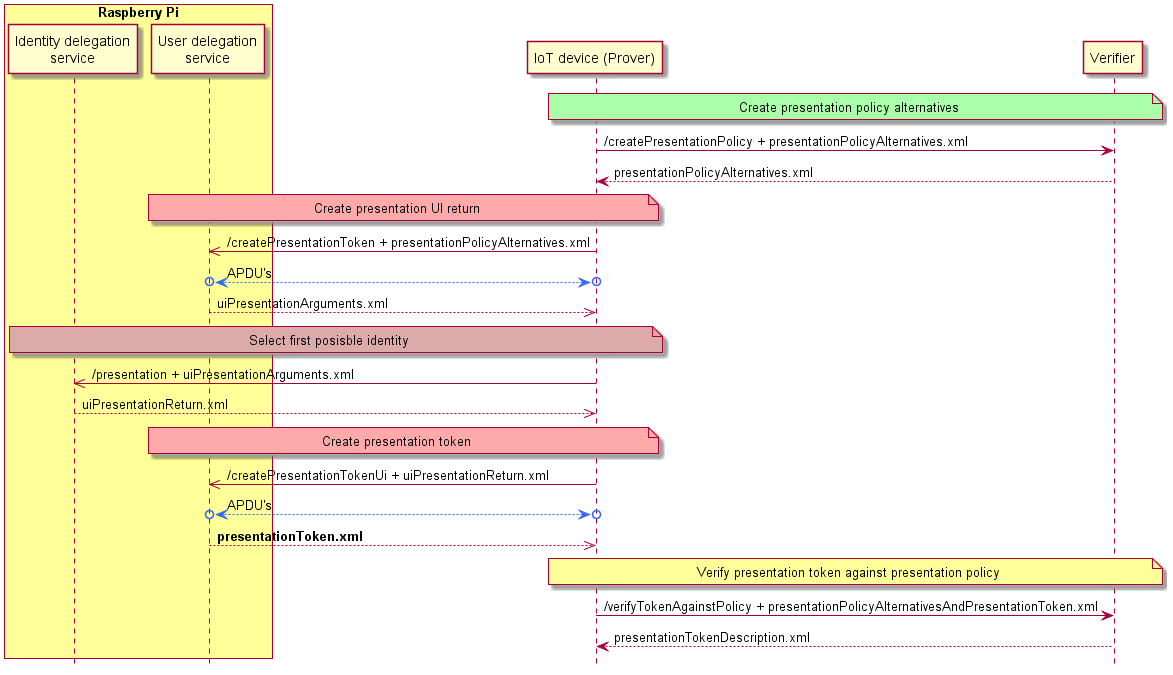
\includegraphics[width=\linewidth]{gfx/UML/ProvingInteraction}
	\end{center}
	\caption{Proving interaction.}
	\label{fig:ProvingInteraction}
\end{figure}



Again, as shown in \autoref{fig:proving:graph}, there is a correlation between the number of APDU Commands used, the work the IoT smart card must perform, and the time measured. The $20$ APDU Commands in the first call make the IoT deployment almost $8$ times slower than the Raspberry Pi 3; but with only $8$ APDU Commands, the second one is less than $1.5$ times slower.

Nonetheless, it's significant the difference in performance between the laptop and the Raspberry Pi 3 in the last REST call, more than $40$ times slower, even using the \textit{SoftwareSmartcard}.


\begin{figure}[bth]
	\myfloatalign
	\subfloat[Times (ms) and relative speedup]
	{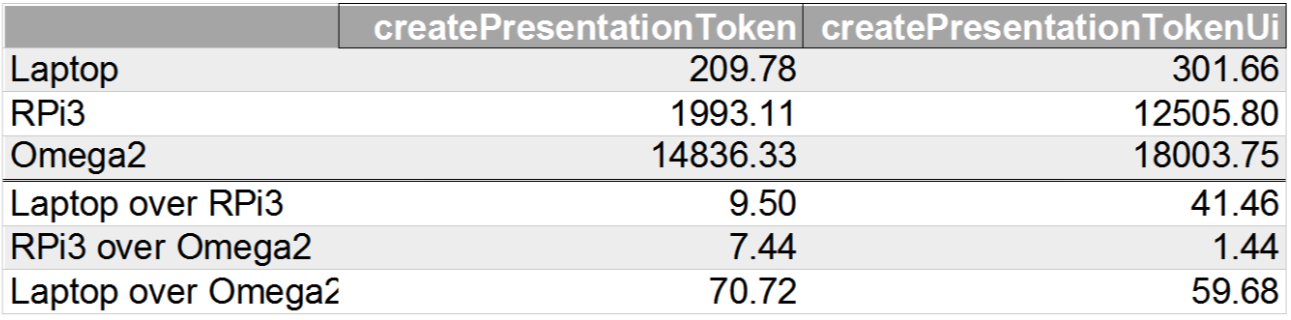
\includegraphics[width=.8\linewidth]{gfx/graphics/provingtable}} \quad
	\subfloat[Comparison graph]
	{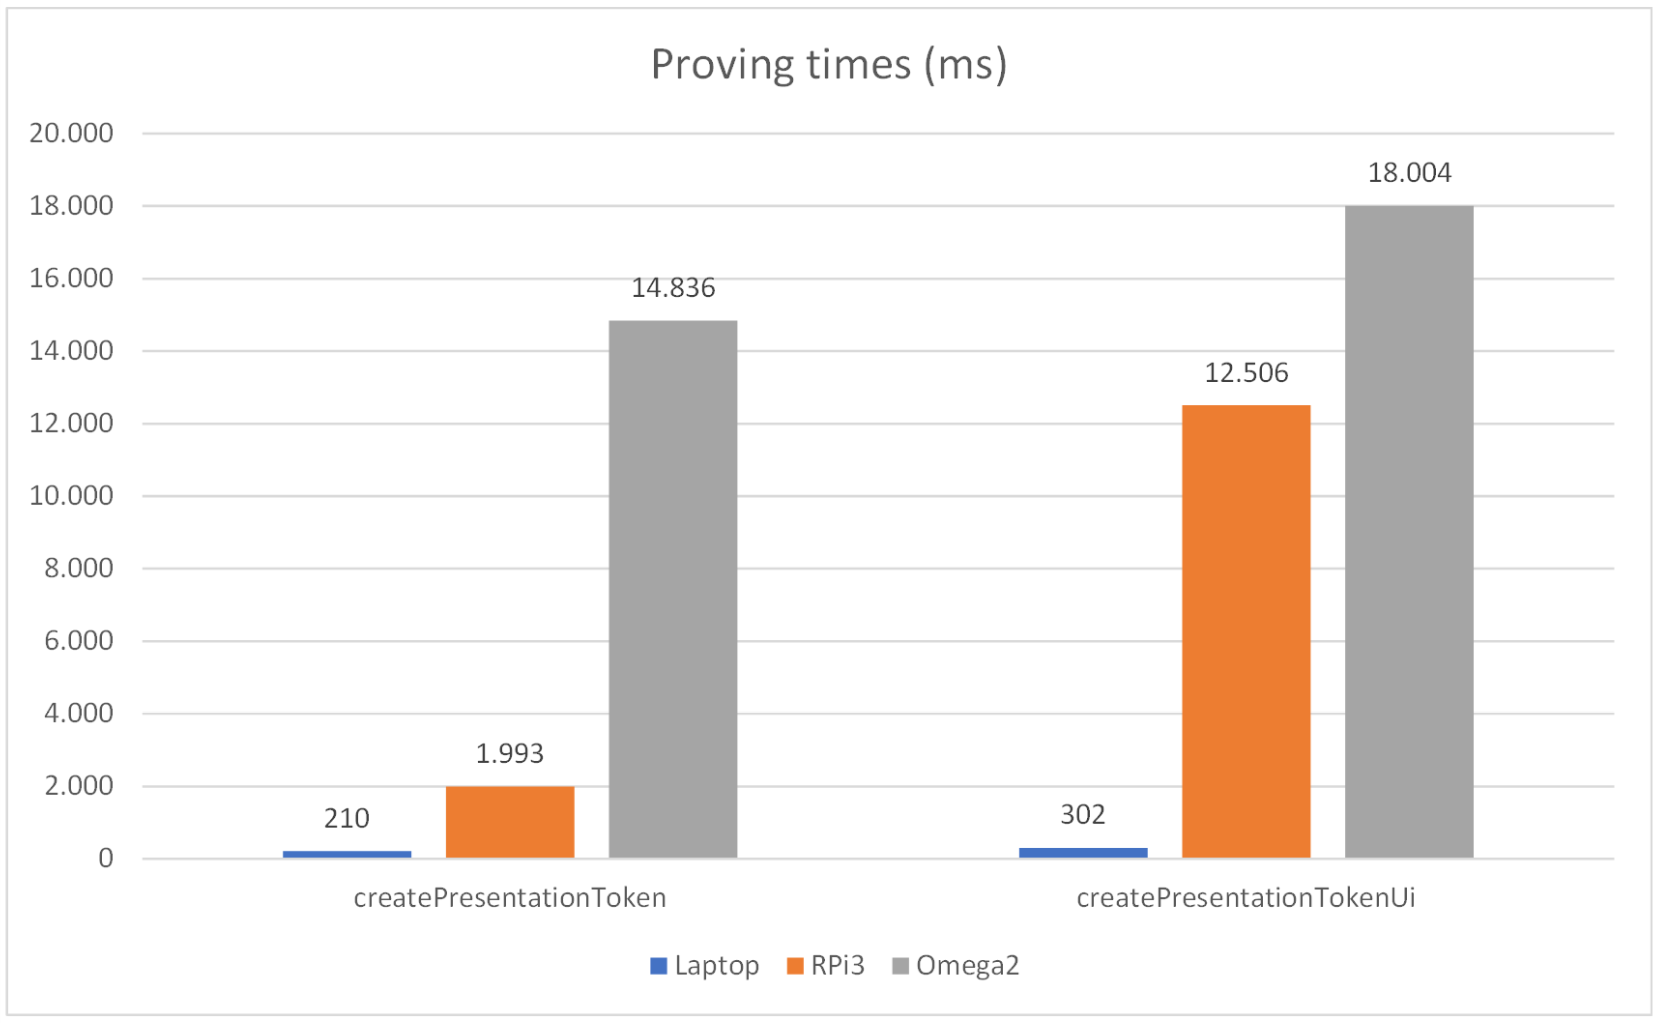
\includegraphics[width=.7\linewidth]{gfx/graphics/proving}} \\
	\caption{Proving times (milliseconds)}
	\label{fig:proving:graph}
\end{figure}

Unlike the previous steps, the Presentation or Proving is done more than once, being the key feature of ZKP protocols. The laptop performs a prove in less than one second, the RPi3 needs $15$ seconds, but our P2ABCE IoT deployment needs $15$ seconds for the first step, and $18$s for the second step, $33$ seconds total to generate a Presentation Token.




\hfil

\paragraph{Memory usage on the Omega2}\hfil

Using the tool \textit{time -v} we can get a lot of useful information about a program, once it finishes. In our case, the binary with BIOSC and the smart card logic starts as an empty smart card, goes through the described process, and then we can stop it, as the User Service won't use it anymore.

After another round of tests, now using \textit{time -v}, the field named \textit{Maximum resident set size (kbytes)} shows the \textbf{maximum} size of RAM used by the process since its launch. In our case, this involves the use of static memory for the \textit{global variables} of the smart card logic, and the dynamic memory used by the third party libraries, like GMPlib, OpenSSL and cJSON.

GMP and OpenSSL always allocate the data in their own ADT, what involves copying the arrays of bytes representing the big modular integers from the cryptographic operations. cJSON, used in the serialization of the smart card for storage, and debug being human readable, stores a copy of every saved variable in the JSON tree structure, then creates a string (array of char) with the JSON, that the user can write to a file.

Understanding the many bad uses of memory done in this PoC is important for future improvements and ports. A custom modular library using the same array of bytes that the smart card logic, a binary serialization, and many improvements, are our future work.

With all that said, the mean of the maximum memory usage measured is $6569.6$ kbytes. Compared to the $64$MB of RAM available in the Omega2, our PoC could be executed in more constrained devices, given the system is compatible.




\section{Validation conclusions}

Below \autoref{totaltime} sums up the time in seconds used in each step of the test for the Omega2 and Raspberry Pi 3 setup.

The first step, \textit{System Setup} is done only once when the system is being deployed, and the \textit{IoT Smart Card Setup} only once per device.

Because a device can have more than one credential, the Issuance step is significant when we issue multiple credentials over the device's lifetime. We recall that our tests used a credential with five attributes and key sizes of 1024 bits.

Finally, the Proving step is expected to be the most performed calculation by the IoT device. The fact that it lasts over half a minute implies that we should not use this PoC for \textit{real-time} applications yet, usually used in critical secure systems. Nevertheless, for many other IoT applications, the fact this operation can be performed multiple times per hour, presents an useful tool for privacy, e.g. the thermostat system mentioned in the smart building, which can pool data from the sensors every few minutes.


\begin{table}[!ht]
	\begin{center}
		\begin{tabular}{|r|r|r|r|}
		\hline
		System & IoT Smart  & Issue  & Prove Presen-\\
		Setup & Card Setup & credential & tation Policy\\ \hline
		3.77 s & 19.19 s & 36.48 s & 32.84 s \\ \hline
	\end{tabular}
	\end{center}
\caption{Total time spent for each step in the Omega2+RPi3 setup.}
\label{totaltime}
\end{table}
